\chapter{Organisation fonctionnelle d'un mammifère}\label{ch:b1:mammal-organization}

Ouvrez un lapin sur la table de dissection et la première impression est
celle de l'ordre. Une nappe musculaire, le \omterm{def:b1:mammal-organization:bodyplan}{diaphragme}, divise le tronc
en un thorax contenant le cœur et deux poumons et un abdomen contenant
tout le reste~: un foie de la taille d'un poing, un estomac, quatre
mètres d'intestin finissant par un cæcum aussi gros que l'estomac, deux
reins contre la paroi dorsale. Chaque \omterm{def:b1:mammal-organization:organ}{organe} a une place, une
vascularisation et une tâche~; aucun ne travaille seul. Ce chapitre
décrit comment le mammifère est bâti en un tout fonctionnel~: son \omterm{def:b1:mammal-organization:bodyplan}{plan
d'organisation}, les \omterm{def:b1:mammal-organization:organ}{appareils} en lesquels ses \omterm{def:b1:mammal-organization:organ}{organes} sont groupés, les
compartiments liquidiens où vivent ses cellules, les \omterm{prop:b1:organism-environment:surfaces}{surfaces d'échange}
par lesquelles il rencontre l'extérieur, et le \omterm{prop:b1:mammal-organization:heatbudget}{bilan thermique} qui le
maintient à \qty{39}{\celsius} dans un champ de janvier.

\section{Le plan d'organisation d'un mammifère}

\begin{definition}[Plan d'organisation]\label{def:b1:mammal-organization:bodyplan}
Le \emph{plan d'organisation}\index{plan d'organisation} d'un animal est
la disposition de ses axes, de ses cavités et de ses \omterm{def:b1:mammal-organization:organ}{organes} que
partagent tous les membres de son groupe. Le plan d'organisation des
mammifères est celui d'un vertébré~: symétrie bilatérale avec une
extrémité céphalique portant l'encéphale et les principaux \omterm{def:b1:mammal-organization:organ}{organes} des
sens (\emph{céphalisation}\index{cephalisation@céphalisation}), un axe dorsal de
vertèbres entourant la moelle épinière, quatre membres, et une cavité
ventrale --- le \emph{cœlome}\index{coelome@cœlome} --- contenant les viscères.
Ce qui est proprement mammalien~: le cœlome est divisé par le
\emph{diaphragme}\index{diaphragme} musculaire en une cavité thoracique
(cœur, poumons) et une cavité abdominale (\omterm{def:b1:mammal-organization:organ}{organes} digestifs, reins,
gonades)~; le corps est couvert de poils~; les jeunes sont nourris de
lait~; la température est régulée.
\end{definition}

\begin{omfigure}
\begin{tikzpicture}
  \node[anchor=south west, inner sep=0] (img) at (0,0)
    {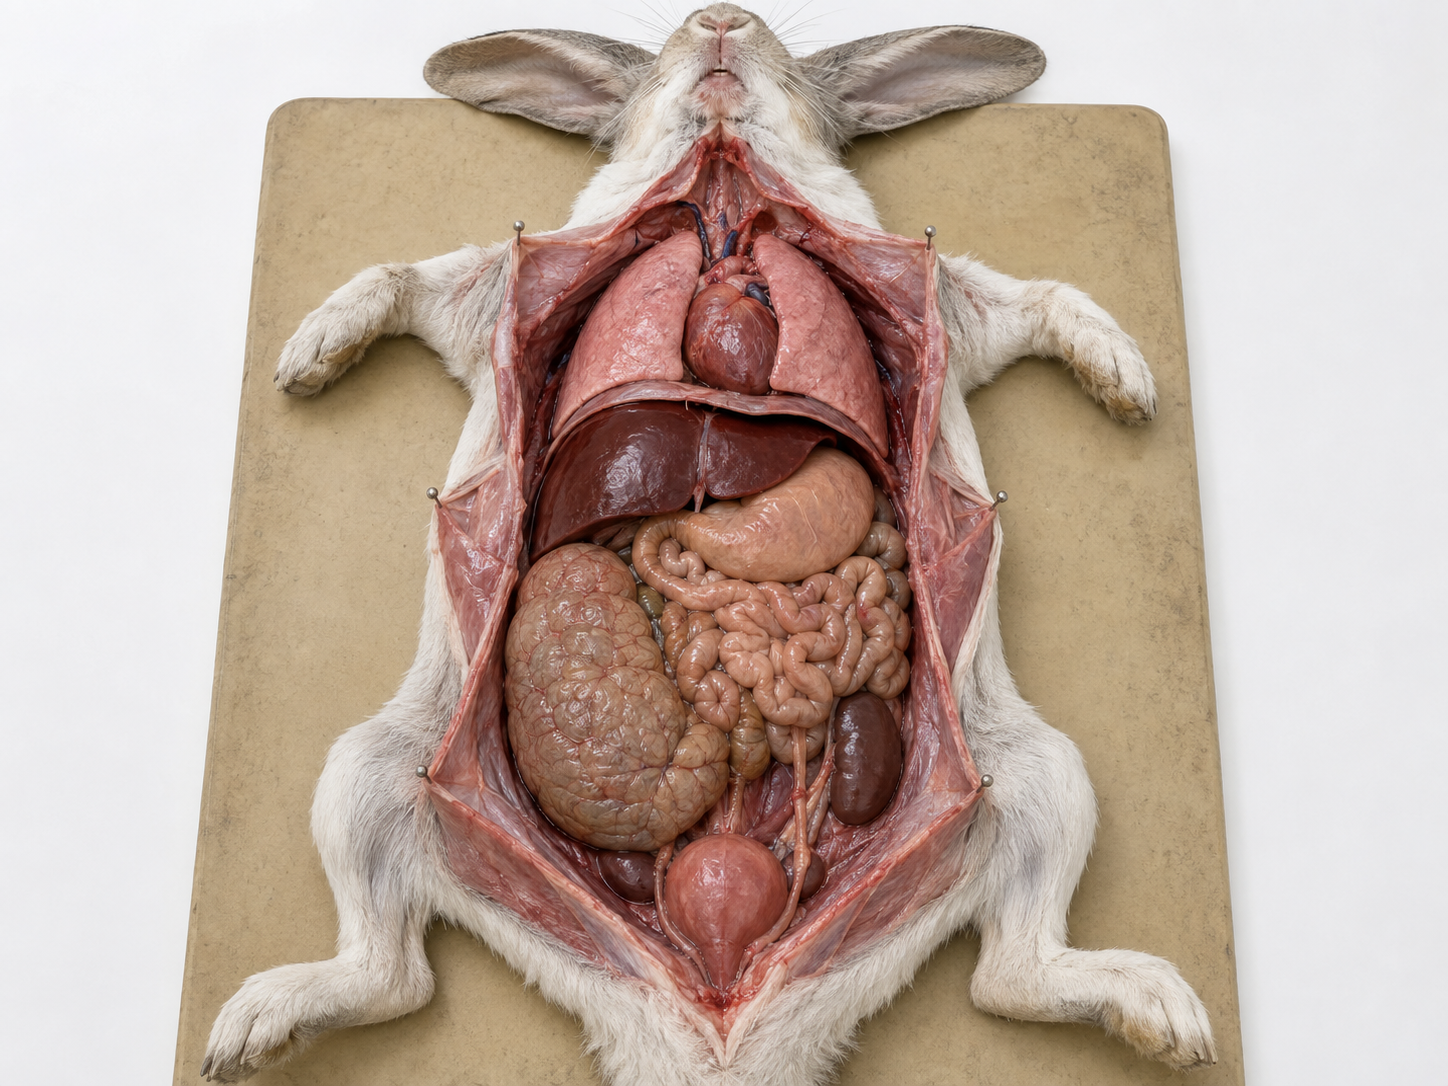
\includegraphics[width=0.6\linewidth]{images/book3/ai/fig-rabbit-dissection.png}};
  \begin{scope}[x={(img.south east)}, y={(img.north west)},
      every node/.style={font=\small}]
    \draw[omDef, thick] (0.44,0.72) -- (-0.02,0.90) node[left] {poumons};
    \draw[omDef, thick] (0.50,0.68) -- (1.02,0.88) node[right] {cœur};
    \draw[omDef, thick] (0.53,0.61) -- (1.02,0.70) node[right] {diaphragme};
    \draw[omDef, thick] (0.44,0.55) -- (-0.02,0.62) node[left] {foie};
    \draw[omDef, thick] (0.56,0.52) -- (1.02,0.54) node[right] {estomac};
    \draw[omDef, thick] (0.52,0.42) -- (1.02,0.40) node[right] {intestin grêle};
    \draw[omDef, thick] (0.42,0.36) -- (-0.02,0.36) node[left] {cæcum};
    \draw[omDef, thick] (0.60,0.30) -- (1.02,0.24) node[right] {rein};
    \draw[omDef, thick] (0.51,0.17) -- (-0.02,0.10) node[left] {vessie};
  \end{scope}
\end{tikzpicture}

{\small Un lapin ouvert par la face ventrale. Le \omterm{def:b1:mammal-organization:bodyplan}{diaphragme} sépare la
cavité thoracique (poumons, cœur) de la cavité abdominale (foie,
estomac, intestin, cæcum, reins, vessie). Chaque \omterm{def:b1:mammal-organization:organ}{organe} occupe une place
fixe, enveloppé d'une membrane et desservi par ses propres vaisseaux.}
\end{omfigure}

\begin{definition}[Organe, appareil]\label{def:b1:mammal-organization:organ}
Un \emph{organe}\index{organe} est une structure faite de plusieurs
tissus (\cref{ch:b1:body-plans-tissues}) disposés pour assurer une
fonction définie~: le cœur pompe, le poumon échange les gaz, le rein
filtre. Un \emph{appareil}\index{appareil} (ou système) est un ensemble
d'organes qui coopèrent à une même grande fonction~: l'appareil digestif
va de la bouche à l'anus, foie et pancréas annexés~; l'appareil
circulatoire, c'est le cœur et les vaisseaux~; l'appareil excréteur, les
reins et les voies urinaires.
\end{definition}

\section{Les appareils et les fonctions qu'ils assurent}

\begin{proposition}[Trois groupes de fonctions]\label{prop:b1:mammal-organization:functions}
Les \omterm{def:b1:mammal-organization:organ}{appareils} d'un mammifère assurent trois groupes de fonctions~:
\begin{itemize}
  \item la \emph{nutrition}\index{fonction de nutrition}~: prélever et
        distribuer matière et énergie et éliminer les déchets ---
        \omterm{def:b1:mammal-organization:organ}{appareils} digestif, respiratoire, circulatoire et excréteur~;
  \item la \emph{relation}\index{fonction de relation}~: percevoir
        l'environnement et agir sur lui --- \omterm{def:b1:mammal-organization:organ}{organes} des sens, système
        nerveux, glandes endocrines, squelette et muscles~;
  \item la \emph{reproduction}\index{fonction de reproduction}~:
        produire une descendance --- gonades, voies génitales et, chez
        les mammifères, glandes mammaires.
\end{itemize}
Aucun \omterm{def:b1:mammal-organization:organ}{appareil} ne travaille seul~: chaque \omterm{def:b1:mammal-organization:organ}{organe} dépend du sang pour son
approvisionnement, des systèmes nerveux et endocrinien pour sa
coordination, et du squelette et de la peau pour sa protection.
\end{proposition}

\begin{omfigure}
\begin{tikzpicture}[font=\footnotesize, >=Stealth, line cap=round,
  sys/.style={draw, thick, rounded corners=3pt, minimum height=7mm, minimum width=24mm, align=center, fill=white},
  lab/.style={font=\scriptsize, above},
  grp/.style={font=\small\bfseries, anchor=west}]
  \node[grp, omProp] at (0,4.6) {Nutrition};
  \node[sys, fill=omProp!12] (dig) at (1.3,3.8) {digestif};
  \node[sys, fill=omProp!12] (res) at (1.3,2.9) {respiratoire};
  \node[sys, fill=omProp!12] (exc) at (1.3,2.0) {excréteur};
  \node[grp, omExo] at (0,1.1) {Reproduction};
  \node[sys, fill=omExo!12] (gen) at (1.3,0.3) {génital};
  \node[sys, fill=omThm!12, minimum height=30mm] (cir) at (5.9,2.6) {circulatoire\\ (sang, lymphe)};
  \node[grp, omDef] at (8.6,4.6) {Relation};
  \node[sys, fill=omDef!12, minimum width=30mm] (ner) at (10.3,3.8) {nerveux, sens};
  \node[sys, fill=omDef!12, minimum width=30mm] (end) at (10.3,2.9) {endocrinien};
  \node[sys, fill=omDef!12, minimum width=30mm] (mus) at (10.3,2.0) {squelette, muscles};
  \node[sys, fill=omDef!12, minimum width=30mm] (ski) at (10.3,1.1) {peau};
  \draw[<->, thick] (dig.east) -- (cir.west |- dig.east) node[lab, midway] {nutriments};
  \draw[<->, thick] (res.east) -- (cir.west |- res.east) node[lab, midway] {$\mathrm{O_2}$, $\mathrm{CO_2}$};
  \draw[<->, thick] (exc.east) -- (cir.west |- exc.east) node[lab, midway] {déchets};
  \draw[<->, thick] (gen.east) -- ++(1.6,0) |- (cir.south west);
  \draw[<->, thick] (cir.east |- ner.west) -- (ner.west);
  \draw[<->, thick] (cir.east |- end.west) -- (end.west) node[lab, midway] {hormones};
  \draw[<->, thick] (cir.east |- mus.west) -- (mus.west);
  \draw[<->, thick] (cir.south east) -| ++(0.5,0) |- (ski.west);
\end{tikzpicture}

{\small Les \omterm{def:b1:mammal-organization:organ}{appareils} d'un mammifère groupés par fonction. La
circulation est le carrefour~: chaque \omterm{def:b1:mammal-organization:organ}{appareil} échange avec le sang, et
le sang porte à tous les autres ce qu'un \omterm{def:b1:mammal-organization:organ}{appareil} a prélevé.}
\end{omfigure}

\begin{example}[Une bouchée d'herbe]\label{ex:b1:mammal-organization:mouthful}
L'herbe du lapin est coupée par les incisives et broyée par les molaires
(squelette et muscles), goûtée et sentie (sens), avalée et digérée dans
l'estomac et l'intestin grêle~; ses sucres et ses acides aminés
traversent la paroi intestinale vers le sang et gagnent le foie, qui les
stocke ou les libère sous contrôle hormonal (endocrinien)~; sa cellulose
est fermentée par des bactéries dans le cæcum~; l'oxygène qui brûlera
les sucres arrive par les poumons, le dioxyde de carbone repart par la
même voie, l'urée issue des acides aminés sort par les reins, et la
chaleur de tout le processus sort par la peau. Sept \omterm{def:b1:mammal-organization:organ}{appareils} pour une
bouchée.
\end{example}

\section{Les compartiments du corps}

\begin{definition}[Compartiments liquidiens]\label{def:b1:mammal-organization:compartments}
L'eau représente environ \qty{60}{\%} de la masse d'un mammifère. Les
deux tiers en sont le \emph{liquide intracellulaire}
\index{liquide intracellulaire}, à l'intérieur des cellules~; le tiers
restant est le
\emph{liquide extracellulaire}\index{liquide extracellulaire}, le \omterm{def:b1:organism-environment:milieu}{milieu
intérieur} du \cref{ch:b1:organism-environment}, lui-même divisé en
\emph{liquide interstitiel}\index{liquide interstitiel} baignant les
cellules (les trois quarts) et en \emph{plasma
sanguin}\index{plasma} contenu dans les vaisseaux (le quart). La
\emph{lymphe}\index{lymphe} est du liquide interstitiel collecté par les
vaisseaux lymphatiques et rendu au sang. Les deux liquides
extracellulaires ont presque la même composition --- le plasma en
diffère par ses protéines, qui ne traversent pas la paroi capillaire ---
et tous deux diffèrent nettement du liquide intracellulaire.
\end{definition}

\begin{omfigure}
\begin{tikzpicture}[font=\small, line cap=round]
  \draw[thick, fill=gray!8, rounded corners=6pt] (0,0) rectangle (11.6,4.6);
  \node[anchor=north west, font=\small\bfseries] at (0.15,4.55) {eau corporelle totale~: \qty{42}{L} (\qty{60}{\%} de \qty{70}{kg})};
  \draw[thick, fill=omDef!14, rounded corners=5pt] (0.3,0.3) rectangle (6.4,3.8);
  \node[anchor=north west, align=left] at (0.4,3.7) {\textbf{liquide intracellulaire}~: \qty{28}{L}\\ riche en $\mathrm{K^+}$ (\qty{140}{mmol/L}),\\ phosphate, protéines~;\\ pauvre en $\mathrm{Na^+}$ (\qty{10}{mmol/L})};
  \draw[thick, fill=omProp!14, rounded corners=5pt] (6.7,0.3) rectangle (11.3,3.8);
  \node[anchor=north west, align=left] at (6.8,3.7) {\textbf{liquide extracellulaire}~: \qty{14}{L}\\ riche en $\mathrm{Na^+}$ (\qty{140}{mmol/L}),\\ $\mathrm{Cl^-}$, $\mathrm{HCO_3^-}$};
  \draw[thick, fill=omProp!30, rounded corners=4pt] (6.9,0.45) rectangle (9.2,1.55);
  \node[align=center, font=\footnotesize] at (8.05,1.0) {interstitiel\\ \qty{11}{L}};
  \draw[thick, fill=omThm!30, rounded corners=4pt] (9.4,0.45) rectangle (11.1,1.55);
  \node[align=center, font=\footnotesize] at (10.25,1.0) {plasma\\ \qty{3}{L}};
\end{tikzpicture}

{\small Les compartiments liquidiens d'un humain de \qty{70}{kg}. Les
deux tiers de l'eau sont à l'intérieur des cellules~; le tiers
extracellulaire, partagé entre le \omterm{def:b1:mammal-organization:compartments}{liquide interstitiel} et le \omterm{def:b1:mammal-organization:compartments}{plasma}, est
le \omterm{def:b1:organism-environment:milieu}{milieu intérieur}. Le sodium domine au-dehors, le potassium au-dedans
--- une différence que chaque cellule dépense de l'énergie à maintenir
(\cref{ch:b1:membranes-transport}).}
\end{omfigure}

\begin{method}[Mesurer un compartiment par dilution]\label{met:b1:mammal-organization:dilution}
\begin{enumerate}
  \item Choisir un marqueur qui se répartit dans le compartiment et
        nulle part ailleurs~: un colorant lié aux protéines
        plasmatiques (bleu Evans) pour le \omterm{def:b1:mammal-organization:compartments}{plasma}~; l'inuline, un sucre
        qui quitte les vaisseaux mais n'entre pas dans les cellules,
        pour le \omterm{def:b1:mammal-organization:compartments}{liquide extracellulaire}~; l'eau lourde pour l'eau
        corporelle totale.
  \item Injecter une quantité connue $m$ et attendre le mélange
        (quelques minutes pour le \omterm{def:b1:mammal-organization:compartments}{plasma}, quelques heures pour l'eau
        totale).
  \item Mesurer la concentration $c$ dans un prélèvement de \omterm{def:b1:mammal-organization:compartments}{plasma}, en
        corrigeant toute perte (urine, métabolisme) survenue pendant
        l'attente.
  \item Le volume vaut $V = m/c$. Le volume intracellulaire est l'eau
        totale moins l'extracellulaire~; le volume interstitiel est
        l'extracellulaire moins le \omterm{def:b1:mammal-organization:compartments}{plasma}. La volémie est le volume
        plasmatique divisé par la fraction plasmatique du sang
        ($1 - $ hématocrite).
\end{enumerate}
\end{method}

\begin{example}[Un volume plasmatique]\label{ex:b1:mammal-organization:evansblue}
\qty{50}{mg} de bleu Evans injectés à un homme de \qty{70}{kg} donnent,
dix minutes plus tard, une concentration plasmatique de
\qty{16.7}{mg/L}~: $V = 50/16.7 = \qty{3.0}{L}$ de \omterm{def:b1:mammal-organization:compartments}{plasma}. Avec un
hématocrite de \qty{45}{\%}, la volémie vaut
$3.0/0.55 = \qty{5.5}{L}$ --- \qty{8}{\%} de la masse corporelle, une
proportion valable de la souris à la baleine.
\end{example}

\section{Surfaces d'échange et circulation}

\begin{proposition}[Toute surface d'échange est couplée au sang]\label{prop:b1:mammal-organization:surfaces}
Un mammifère échange avec l'extérieur par quatre surfaces, chacune
repliée dans le corps et chacune irriguée par un réseau capillaire
dense~: la muqueuse intestinale (\qty{30}{m^2} chez l'humain) pour les
nutriments et l'eau, la surface alvéolaire des poumons
(\qty{100}{m^2}) pour l'oxygène et le dioxyde de carbone, la surface
filtrante des reins (un million de glomérules, filtrant \qty{180}{L} de
\omterm{def:b1:mammal-organization:compartments}{plasma} par jour) pour les déchets et la régulation du \omterm{def:b1:organism-environment:milieu}{milieu intérieur},
et la peau (\qty{2}{m^2}) pour la chaleur et un peu d'eau. La
circulation les relie~: le sang qui quitte une surface atteint la
suivante en moins d'une minute, de sorte que ce qui entre par
l'intestin est oxydé avec l'oxygène du poumon et que son déchet sort par
le rein.
\end{proposition}

\begin{omfigure}
\begin{tikzpicture}[font=\small, >=Stealth, line cap=round,
  org/.style={draw, thick, rounded corners=4pt, minimum height=8mm, minimum width=22mm, align=center, fill=white}]
  \node[org, fill=omDef!12] (lung) at (0,3.2) {poumons\\ \qty{100}{m^2}};
  \node[org, fill=omThm!15, minimum width=26mm, minimum height=12mm] (heart) at (0,0) {cœur\\ droit $\mid$ gauche};
  \node[org, fill=omProp!12] (gut) at (5.2,1.6) {intestin\\ \qty{30}{m^2}};
  \node[org, fill=omProp!12] (liver) at (5.2,0.0) {foie};
  \node[org, fill=omProp!12] (kid) at (5.2,-1.6) {reins\\ \qty{180}{L/d}};
  \node[org, fill=omExo!12] (mus) at (5.2,3.2) {muscles, peau,\\ encéphale, autres};
  % pulmonary loop
  \draw[->, very thick, omDef] (heart.north west) ++(-0.2,0) |- (lung.west) node[pos=0.25, left, font=\footnotesize, align=right] {circulation\\ pulmonaire};
  \draw[->, very thick, omThm] (lung.east) -| ($(heart.north east)+(0.2,0)$);
  % systemic loop: left heart -> organs (parallel) -> right heart
  \draw[very thick, omThm] (heart.east) -- ++(1.2,0) coordinate (a);
  \draw[->, very thick, omThm] (a) |- (mus.west);
  \draw[->, very thick, omThm] (a) |- (gut.west);
  \draw[->, very thick, omThm] (a) |- (kid.west);
  \draw[->, very thick, omThm] (a) -- (liver.west);
  \draw[->, very thick, omDef] (gut.south) -- (liver.north) node[midway, right, font=\footnotesize] {veine porte};
  \coordinate (b) at (8.0,0.8);
  \draw[very thick, omDef] (mus.east) -| (b);
  \draw[very thick, omDef] (liver.east) -| (b);
  \draw[very thick, omDef] (kid.east) -| (b);
  \draw[->, very thick, omDef] (b) |- ++(0,-3.2) -| (heart.south) node[pos=0.25, below, font=\footnotesize] {circulation systémique~: veines};
\end{tikzpicture}

{\small La double circulation d'un mammifère. Le cœur droit envoie le
sang pauvre en oxygène (bleu) vers les poumons~; le cœur gauche envoie
le sang oxygéné (rouge) vers les \omterm{def:b1:mammal-organization:organ}{organes}, disposés en parallèle, de
sorte que chacun reçoit du sang artériel frais. Le sang venu de
l'intestin traverse le foie avant de revenir au cœur.}
\end{omfigure}

\begin{omfigure}
\begin{tikzpicture}
\begin{axis}[
  xbar, bar width=8pt,
  width=0.82\linewidth, height=6.2cm,
  axis x line=bottom, axis y line=left,
  xmin=0, xmax=1.8, xlabel={débit sanguin au repos (\unit{L/min})},
  xlabel style={font=\small, at={(axis description cs:0.5,-0.13)}, anchor=north},
  symbolic y coords={muscle cardiaque, peau, encéphale, muscles squelettiques, reins, foie et intestin},
  ytick=data, tick label style={font=\small},
  enlarge y limits=0.12, xtick={0,0.5,1.0,1.5},
  nodes near coords, nodes near coords style={font=\scriptsize, anchor=west},
]
\addplot[fill=omThm!45, draw=omThm] coordinates
  {(0.25,muscle cardiaque) (0.4,peau) (0.75,encéphale) (1.0,muscles squelettiques) (1.1,reins) (1.35,foie et intestin)};
\end{axis}
\end{tikzpicture}

{\small Comment un débit cardiaque humain de \qty{5}{L/min} au repos se
partage entre les \omterm{def:b1:mammal-organization:organ}{organes}. Les reins, \qty{0.5}{\%} de la masse
corporelle, en prennent le cinquième --- le prix à payer pour filtrer
tout le \omterm{def:b1:mammal-organization:compartments}{plasma} soixante fois par jour. À l'effort, la part des muscles
est multipliée par dix et celle de l'intestin diminue.}
\end{omfigure}

\begin{example}[Le temps de circulation]\label{ex:b1:mammal-organization:circtime}
Avec \qty{5.5}{L} de sang et un débit cardiaque de \qty{5}{L/min}, une
goutte de sang boucle le double circuit en une minute environ au repos,
et en un quart de ce temps à l'effort intense, quand le débit atteint
\qty{20}{L/min}. Le débit cardiaque varie en $M^{3/4}$
(\cref{thm:b1:organism-environment:kleiber})~: celui d'un lapin de
\qty{2}{kg} vaut environ \qty{0.35}{L/min} pour \qty{160}{mL} de sang
--- le même temps de circulation à un facteur deux près, avec une
fréquence cardiaque de \qty{200}{} battements par minute.
\end{example}

\section{Endothermie et bilan thermique}

\begin{proposition}[Le bilan thermique]\label{prop:b1:mammal-organization:heatbudget}
\index{bilan thermique}
Un mammifère à température stationnaire vérifie
\[
M - W = R + C + K + E ,
\]
où $M$ est la production métabolique de chaleur, $W$ le travail
mécanique fourni à l'extérieur, et le membre de droite les pertes par
rayonnement $R$, convection vers l'air $C$, conduction vers le sol $K$
et évaporation $E$ (par les poumons, et par la sueur ou le halètement).
Les trois premières pertes sont proportionnelles à $T_b - T_a$ et sont
gouvernées par l'isolation du pelage et par le débit sanguin cutané~;
l'évaporation est la seule voie qui fonctionne encore quand l'air est
plus chaud que le corps. Lorsque l'équation n'est pas vérifiée, la
température corporelle dérive à une vitesse fixée par le déséquilibre et
par la capacité thermique du corps (environ
\qty{3.5}{kJ.kg^{-1}.K^{-1}}).
\end{proposition}
\begin{proof}
Conservation de l'énergie pour le corps sur une période où sa
température ne change pas~: l'énergie chimique libérée ($M$) sort sous
forme de travail ou de chaleur par les quatre canaux physiques. La
proportionnalité de $R$, $C$, $K$ à l'écart de température est la loi de
refroidissement de Newton (\cref{ch:b1:organism-environment})~;
l'indépendance de $E$ vis-à-vis de cet écart tient à ce que
l'évaporation est entraînée par le gradient d'humidité et non par le
gradient de température.
\end{proof}

\begin{omfigure}
\begin{tikzpicture}[font=\small, >=Stealth, line cap=round]
  \draw[very thick, fill=omThm!8, rounded corners=16pt] (0,0) rectangle (5.0,3.0);
  \node[align=center] at (2.5,1.5) {noyau central \qty{39}{\celsius}\\ production de chaleur $M$\\ (basale, frisson, activité)};
  \draw[->, very thick, omThm] (5.0,2.5) -- (6.6,2.5) node[right, align=left] {$R$~: rayonnement (parois, ciel)};
  \draw[->, very thick, omThm] (5.0,1.8) -- (6.6,1.8) node[right, align=left] {$C$~: convection vers l'air};
  \draw[->, very thick, omThm] (5.0,1.1) -- (6.6,1.1) node[right, align=left] {$K$~: conduction vers le sol};
  \draw[->, very thick, omDef] (5.0,0.4) -- (6.6,0.4) node[right, align=left] {$E$~: évaporation (souffle, sueur)};
  \draw[->, very thick, omExo] (-1.6,1.5) -- (0,1.5) node[pos=0, left, align=right] {énergie alimentaire\\ (et graisse stockée)};
  \draw[->, very thick, gray] (2.5,0) -- (2.5,-0.9) node[below, align=center] {$W$~: travail fourni à l'extérieur};
  \node[font=\footnotesize, align=center, anchor=south] at (2.5,3.1) {pelage et débit cutané fixent $R$, $C$, $K$~;\\ ils sont $\propto (T_b - T_a)$};
\end{tikzpicture}

{\small Le \omterm{prop:b1:mammal-organization:heatbudget}{bilan thermique} d'un \omterm{prop:b1:organism-environment:thermo}{endotherme}. La production doit égaler la
somme des quatre pertes augmentée du travail extérieur~; l'animal ajuste
sa production (frisson, activité), son isolation (pelage, posture, débit
cutané) et son évaporation pour maintenir l'équilibre.}
\end{omfigure}

\begin{proposition}[Les moyens de la thermorégulation]\label{prop:b1:mammal-organization:thermoreg}
Contre le froid, un mammifère réduit ses pertes --- hérissement du
pelage, vasoconstriction cutanée et des extrémités, position en boule,
regroupement --- et augmente sa production~: le frisson (contraction
rythmique des muscles) et, chez les petits mammifères et les jeunes, la
\emph{thermogenèse sans frisson}\index{thermogenese sans frisson@thermogenèse sans frisson} dans
le \emph{tissu adipeux brun}\index{tissu adipeux brun}, dont les
mitochondries libèrent directement en chaleur l'énergie des graisses.
Contre la chaleur, il dilate les vaisseaux cutanés (les oreilles d'un
lapin peuvent évacuer le tiers de sa chaleur) et évapore de l'eau par
sudation (cheval, humain) ou par halètement (chien, lapin). Tout cela
est commandé depuis l'hypothalamus, qui détient la \omterm{def:b1:organism-environment:homeostasis}{valeur de consigne} et
lit la température du sang et celle de la peau.
\end{proposition}
\begin{proof}[Faits expérimentaux]
Réchauffer l'hypothalamus d'un chien au moyen d'une sonde implantée le
fait haleter et dilater ses vaisseaux cutanés dans une pièce froide~;
refroidir la sonde le fait frissonner dans une pièce chaude. La
consommation d'oxygène d'un rat placé à \qty{5}{\celsius} triple en une
heure, la moitié de l'augmentation venant du frisson (enregistré comme
activité électrique musculaire) et l'autre moitié de la graisse brune,
dont la température, mesurée au thermocouple, dépasse celle des tissus
voisins. Des images infrarouges d'un lapin à \qty{30}{\celsius}
montrent ses oreilles presque à la température du corps, et à
\qty{5}{\celsius} presque à celle de l'air.
\end{proof}

\begin{example}[Les oreilles du lapin]\label{ex:b1:mammal-organization:ears}
Deux oreilles d'environ \qty{50}{cm^2} chacune, minces, presque nues et
richement vascularisées~: vaisseaux ouverts, à \qty{30}{\celsius} dans
un air à \qty{20}{\celsius}, avec un coefficient de peau nue de
\qty{10}{W.m^{-2}.K^{-1}}, elles perdent $10\times 0.01\times 10 =
\qty{1}{W}$, le sixième de la production d'un lapin au repos. À
\qty{5}{\celsius} les vaisseaux se ferment, les oreilles refroidissent
jusqu'à la température de l'air, et la perte par leur intermédiaire
tombe sous \qty{0.2}{W}.
\end{example}

\begin{remark}[Coordination]\label{rem:b1:mammal-organization:coordination}
Chacun des ajustements ci-dessus --- un vaisseau qui se rétrécit, un
muscle qui frissonne, une glande qui sécrète --- est une commande portée
par un nerf ou par une hormone. Le système nerveux agit en quelques
millisecondes le long de câbles fixes~; le système endocrinien agit en
quelques minutes à quelques heures par le sang, atteignant toute cellule
qui porte le bon récepteur. Leurs mécanismes font l'objet du volume de
deuxième année~; cette année les tient pour acquis et étudie ce qu'ils
coordonnent.
\end{remark}

\section{Exercices}

\begin{exercise}[$\star$]\label{exo:b1:mammal-organization:1}
Énumérer les caractères du \omterm{def:b1:mammal-organization:bodyplan}{plan d'organisation} des mammifères qui sont
partagés par tous les vertébrés, et ceux qui sont propres aux
mammifères.
\end{exercise}

\begin{exercise}[$\star$]\label{exo:b1:mammal-organization:2}
Rattacher chaque \omterm{def:b1:mammal-organization:organ}{appareil} à l'un des trois groupes de fonctions, et
nommer un \omterm{def:b1:mammal-organization:organ}{organe} de chaque \omterm{def:b1:mammal-organization:organ}{appareil}.
\end{exercise}

\begin{exercise}[$\star$]\label{exo:b1:mammal-organization:3}
Une femme de \qty{60}{kg}~: estimer son eau corporelle totale, ses
volumes intracellulaire et extracellulaire, son volume interstitiel et
son volume plasmatique.
\end{exercise}

\begin{exercise}[$\star$]\label{exo:b1:mammal-organization:4}
D'après la figure des débits sanguins, quelle fraction du débit
cardiaque va aux reins, et combien de fois par jour la volémie entière
(\qty{5.5}{L}) y est-elle pompée~?
\end{exercise}

\begin{exercise}[$\star\star$]\label{exo:b1:mammal-organization:5}
On injecte \qty{2.0}{g} d'inuline à un homme de \qty{70}{kg}~; après
mélange, et après que \qty{0.3}{g} a été perdu dans les urines, la
concentration plasmatique vaut \qty{0.12}{g/L}. Calculer le volume
extracellulaire, puis, l'eau totale valant \qty{42}{L}, le volume
intracellulaire.
\end{exercise}

\begin{exercise}[$\star\star$]\label{exo:b1:mammal-organization:6}
Expliquer pourquoi le \omterm{def:b1:mammal-organization:compartments}{plasma} et le \omterm{def:b1:mammal-organization:compartments}{liquide interstitiel} ont la même
composition ionique mais diffèrent par leur teneur en protéines, et ce
qu'il adviendrait du volume interstitiel si les protéines plasmatiques
étaient perdues.
\end{exercise}

\begin{exercise}[$\star\star$]\label{exo:b1:mammal-organization:7}
Pourquoi les \omterm{def:b1:mammal-organization:organ}{organes} du circuit systémique sont-ils disposés en
parallèle plutôt qu'en série~? Quelle serait la conséquence de placer
l'encéphale en aval des muscles~?
\end{exercise}

\begin{exercise}[$\star\star$]\label{exo:b1:mammal-organization:8}
Un humain au repos ($M = \qty{80}{W}$, $W = 0$) dans un air à
\qty{20}{\celsius} perd \qty{20}{W} par évaporation pulmonaire et
cutanée. Si le rayonnement, la convection et la conduction valent
ensemble $hS(T_b - T_a)$ avec $S = \qty{1.8}{m^2}$ et $T_b$ (peau) $=
\qty{33}{\celsius}$, trouver $h$. Qu'advient-il de la température
cutanée lorsque l'air atteint \qty{33}{\celsius}~?
\end{exercise}

\begin{exercise}[$\star\star$]\label{exo:b1:mammal-organization:9}
Un humain à l'effort produit \qty{800}{W} et fournit \qty{200}{W} de
travail extérieur. Les pertes non évaporatives valent \qty{150}{W}.
Quelle masse d'eau doit s'évaporer par heure pour maintenir la
température constante (chaleur latente \qty{2.4}{kJ/g})~? Si la sudation
cesse, à quelle vitesse la température monte-t-elle (\qty{70}{kg},
\qty{3.5}{kJ.kg^{-1}.K^{-1}})~?
\end{exercise}

\begin{exercise}[$\star\star\star$]\label{exo:b1:mammal-organization:10}
Les mammifères nouveau-nés et les petites espèces comptent sur la
graisse brune plutôt que sur le frisson. Proposer deux raisons, à
l'aide du rapport surface/volume et de la nature de chaque mécanisme.
\end{exercise}

\begin{exercise}[$\star\star\star$]\label{exo:b1:mammal-organization:11}
On réchauffe l'hypothalamus d'un chien avec une sonde alors que le chien
se tient dans une pièce froide. Prédire ses réponses, et sa température
centrale au bout d'une heure. Prédire ensuite les réponses d'un chien
dont l'hypothalamus est détruit, placé successivement dans une pièce
froide puis dans une pièce chaude.
\end{exercise}

\begin{exercise}[$\star\star\star$]\label{exo:b1:mammal-organization:12}
«~Le \omterm{def:b1:organism-environment:milieu}{milieu intérieur} est l'océan privé du mammifère.~» Discuter cette
image en un paragraphe~: ce qu'est le \omterm{def:b1:mammal-organization:compartments}{liquide extracellulaire}, ce qui le
maintient constant, et quels \omterm{def:b1:mammal-organization:organ}{appareils} en sont les rivages.
\end{exercise}

\section{Problème~: la journée d'un lapin}

\begin{problem}[{Problème du week-end --- vingt-quatre heures d'un lapin
de deux kilogrammes en janvier~: son énergie, son eau, son sang et sa
chaleur, jusqu'à sa dépense énergétique et son renouvellement d'eau
quotidiens}]
\label{pb:b1:mammal-organization:1}
Un lapin de garenne a une masse de \qty{2.0}{kg} et une température
corporelle de \qty{39}{\celsius}. Son \omterm{def:b1:organism-environment:allometry}{métabolisme basal} suit la \omterm{thm:b1:organism-environment:kleiber}{loi de
Kleiber}, $B = \qty{3.4}{W}\,(M/\qty{1}{kg})^{3/4}$. Sa journée~:
\qty{12}{h} au repos dans son terrier, dans sa \omterm{prop:b1:organism-environment:thermo}{zone de neutralité
thermique}, \qty{6}{h} de recherche de nourriture à trois fois son
\omterm{def:b1:organism-environment:allometry}{métabolisme basal}, et \qty{6}{h} de repos dehors à \qty{5}{\celsius}, où
il doit produire deux fois son \omterm{def:b1:organism-environment:allometry}{métabolisme basal}. Il mange de l'herbe
fraîche contenant \qty{25}{\%} de matière sèche~; la matière sèche
renferme \qty{18}{kJ/g}, dont il digère \qty{65}{\%}.

\medskip
\noindent\textbf{Partie I --- L'énergie.}
\begin{enumerate}
  \item Calculer le \omterm{def:b1:organism-environment:allometry}{métabolisme basal} du lapin, en watts.
  \item Calculer l'énergie dépensée pendant chacune des trois périodes,
        en kilojoules.
  \item Calculer la dépense énergétique quotidienne et l'exprimer comme
        un multiple du \omterm{def:b1:organism-environment:allometry}{métabolisme basal} sur \qty{24}{h}.
  \item Calculer l'énergie digestible d'un gramme d'herbe fraîche.
  \item Calculer la masse d'herbe fraîche mangée par jour, et la masse
        de matière sèche qu'elle contient.
  \item Exprimer la prise fraîche en fraction de la masse corporelle.
  \item En prenant \qty{20}{kJ} par litre d'oxygène consommé, calculer
        la consommation quotidienne d'oxygène et le débit moyen en
        millilitres par minute.
  \item Avec un quotient respiratoire de $0.9$ (litres de
        $\mathrm{CO_2}$ par litre d'$\mathrm{O_2}$), calculer le rejet
        quotidien de dioxyde de carbone en litres et en grammes
        (\qty{22.4}{L/mol}, \qty{44}{g/mol}).
\end{enumerate}

\medskip
\noindent\textbf{Partie II --- L'eau.}
L'oxydation de la matière sèche digérée fournit \qty{0.6}{g} d'eau
métabolique par gramme. La matière sèche non digérée sort dans des
fèces qui contiennent \qty{40}{\%} d'eau. L'urine représente
\qty{130}{mL} par jour. Le lapin respire \qty{860}{L} d'air par jour~;
il inspire un air à \qty{10}{\celsius} contenant \qty{5}{g/m^3} de
vapeur d'eau et expire un air saturé à \qty{37}{\celsius},
\qty{44}{g/m^3}. L'évaporation cutanée vaut \qty{20}{g} par jour.
\begin{enumerate}[resume]
  \item Calculer l'eau apportée par l'herbe.
  \item Calculer l'eau métabolique produite.
  \item Calculer la masse des fèces et l'eau qu'elles emportent.
  \item Calculer l'eau perdue dans le souffle.
  \item Dresser le bilan hydrique~: total des entrées, total des
        sorties, et différence.
  \item Le lapin doit-il boire~? Que devient la différence~?
  \item En août l'herbe est à \qty{50}{\%} de matière sèche. Recalculer
        l'eau apportée par la nourriture pour la même prise
        énergétique, et conclure.
\end{enumerate}

\medskip
\noindent\textbf{Partie III --- Sang et compartiments.}
\begin{enumerate}[resume]
  \item Calculer l'eau corporelle totale du lapin, son volume
        extracellulaire et son volume plasmatique, à l'aide des
        fractions du chapitre.
  \item On injecte \qty{1.5}{mg} de bleu Evans~; la concentration
        plasmatique après mélange vaut \qty{15}{mg/L}. Calculer le
        volume plasmatique et le comparer à l'estimation.
  \item Avec un hématocrite de \qty{40}{\%}, calculer la volémie.
  \item Le débit cardiaque varie en $M^{3/4}$ à partir d'une valeur
        humaine de \qty{5}{L/min} à \qty{70}{kg}. Calculer le débit
        cardiaque du lapin et le temps que met une goutte de sang pour
        boucler le circuit.
  \item Avec une fréquence cardiaque de \qty{200}{} battements par
        minute, calculer le volume d'éjection systolique.
\end{enumerate}

\medskip
\noindent\textbf{Partie IV --- La chaleur.}
La surface du lapin vaut $S = \qty{0.1}{m^2}\,(M/\qty{1}{kg})^{2/3}$~;
son pelage donne $h = \qty{2.5}{W.m^{-2}.K^{-1}}$~; chaque oreille
représente \qty{50}{cm^2} de peau presque nue avec
$h = \qty{10}{W.m^{-2}.K^{-1}}$.
\begin{enumerate}[resume]
  \item Calculer la surface du lapin.
  \item Calculer la chaleur perdue à travers le pelage à
        \qty{5}{\celsius} et la comparer à la production supposée pour
        la période passée dehors.
  \item Calculer la perte par les deux oreilles si leurs vaisseaux sont
        ouverts (peau à \qty{39}{\celsius}) et s'ils sont fermés (peau à
        \qty{8}{\celsius}). Que fait le lapin en janvier~?
  \item En août, à \qty{30}{\celsius}, calculer la perte par le pelage
        et par les oreilles ouvertes, et comparer leur somme à la
        production basale. Comment le lapin se maintient-il à
        \qty{39}{\celsius}~?
  \item Énoncer le résultat~: la dépense énergétique quotidienne du
        lapin en mégajoules, comme multiple de son \omterm{def:b1:organism-environment:allometry}{métabolisme basal}, et
        son renouvellement d'eau quotidien en grammes et en fraction de
        sa masse.
\end{enumerate}
\end{problem}
